\section{Contour Labeling}

We use both image and depth cues to infer the labels of edge pixels. We start with a set 
of edge pixels obtained from an edge detection algorithm and the goal is to assign one 
of the four labels to each of these edge pixels. However, to improve computational efficiency 
and to overcome noise in the data, we link similar connected edge pixels in a neighborhood 
into contour segments. The process is carried out using an edge linking algorithm that 
combines connected edge pixels into a link as long as the curvature of the link is within 
a threshold. Each edge pixel is uniquely mapped to one of the contour segments. Each contour 
segment $c_i$ corresponds to a set of edge pixels and labeling the contour segments will 
uniquely label the edge pixels as well. The problem is thus reduced to computing an optimal 
labeling of all the contour segments. 
The individual steps in the algorithm is shown in Figure~\ref{fig:pipeline}.
\begin{figure}[t]
\centering
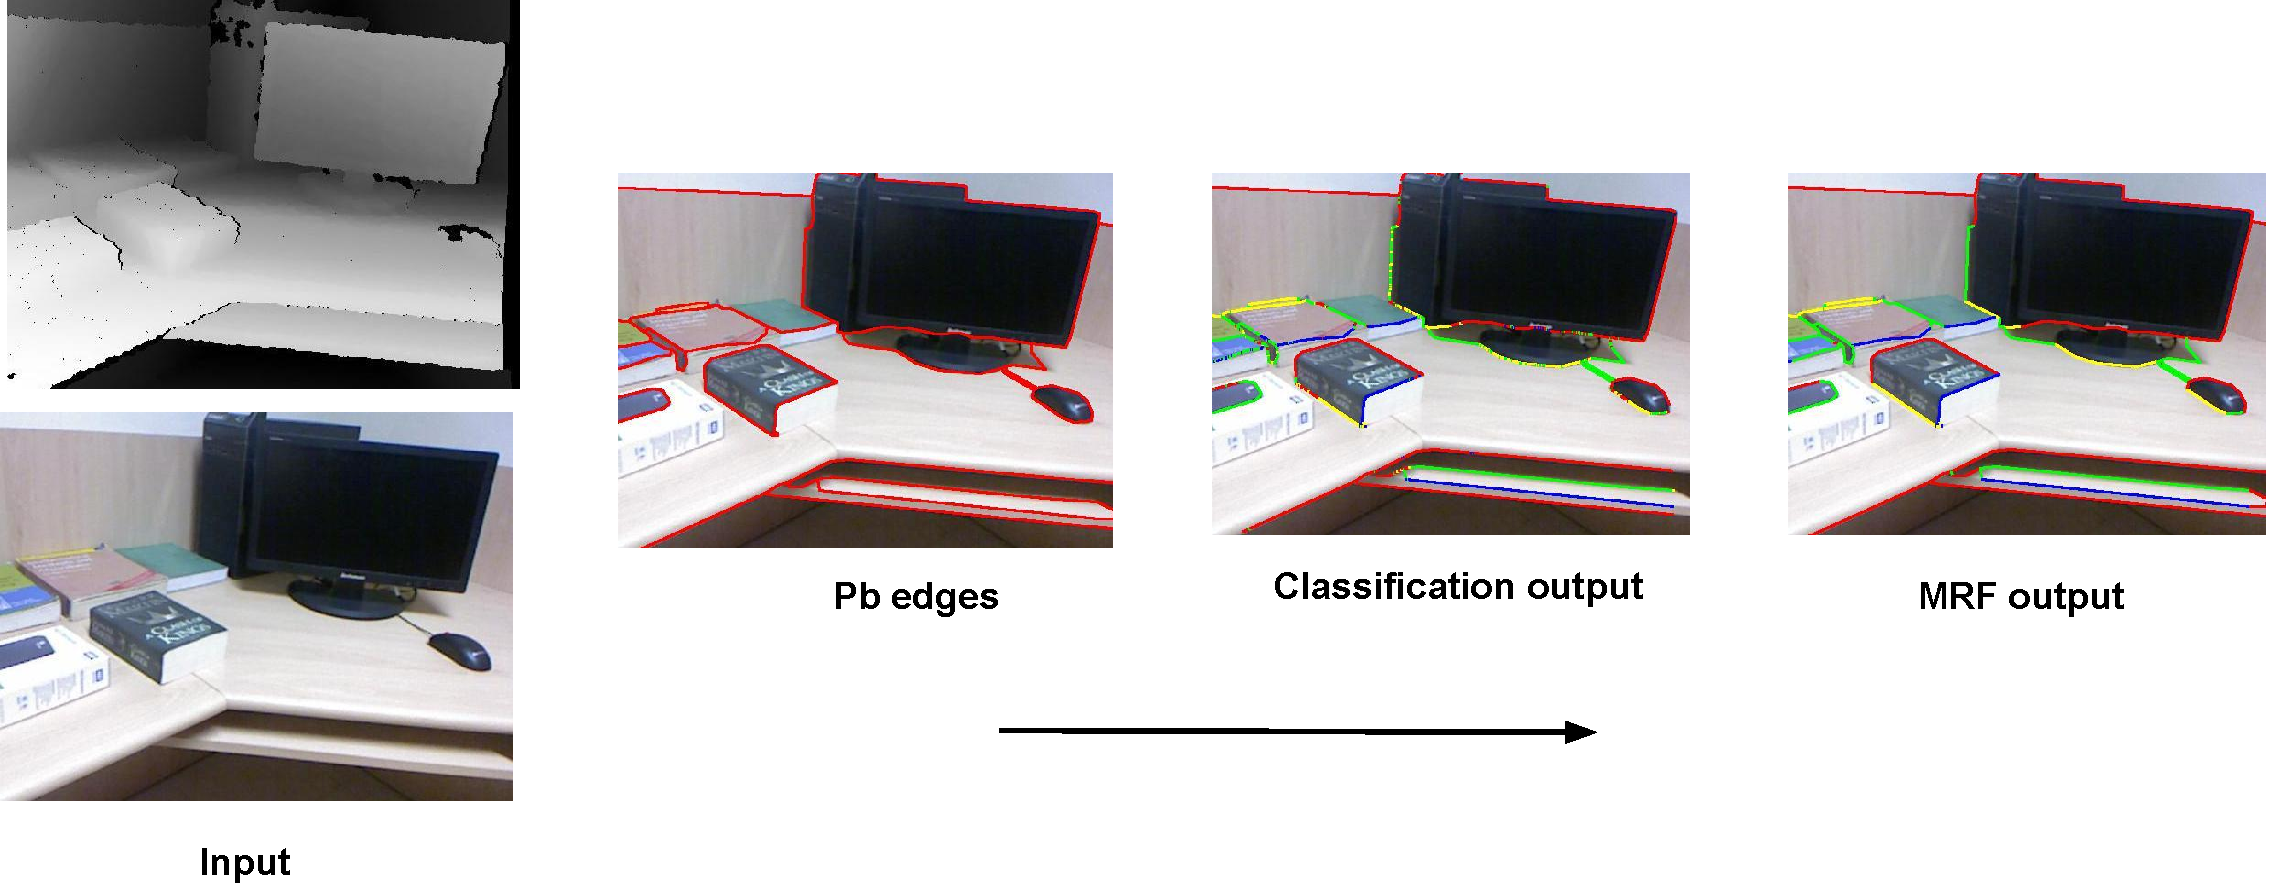
\includegraphics[width=1.0\linewidth]{pipeline_abstract.pdf}
\caption{\it This figure summarizes the pipeline of our approach. It shows RGB and depth maps 
as input (1st image set), with Pb edge detection~\cite{martin2004} (2nd image). The classification and MRF 
outputs are shown in the last two images respectively. Color code: red (occ), green (pln), 
blue (cvx), yellow (ccv).}
\vspace{-2mm}
\label{fig:pipeline}
\end{figure}

\subsection{Contour graph}

Each contour segment is considered as a single entity for 
labeling and is represented as a node in a graph. The junctions between the contour 
segments provide the connectivity information for the graph. Labeling of an object 
boundary is then reduced to labeling of all the nodes in the graph that correspond to 
that specific boundary. Figure~\ref{fig:graph_construction} shows an example, where 
the edge map from a portion of an image is converted into the corresponding contour
graph representation.

We formulate the edge labeling problem as an inference in a graph where the nodes take 
different labels or states. The optimum labeling is achieved by minimizing an energy 
function. Each node can take one of the four labels given by occluding, planar, convex, 
and concave.

Let us consider a graph ${\cal G}=\{{\cal V},{\cal E}\}$, where the vertices of the graph 
correspond to the set of $n$ contour segments; i.e., $c_i \in {\cal V},i=\{1,...,n\}$. The 
edges in the graph are pairs of contour segments. For every junction $J_k$ that falls on 
two contour segments $c_i$ and $c_j$, we have an edge $(c_i,c_j) \in {\cal E}$. Each 
vertex $c_i$ can take four possible states given by ${\cal L}=\{$occ$,$pln$,$cvx$,$ccv$\}$.

\begin{figure}[t]
       \centering
       \subfigure[Edge Links]{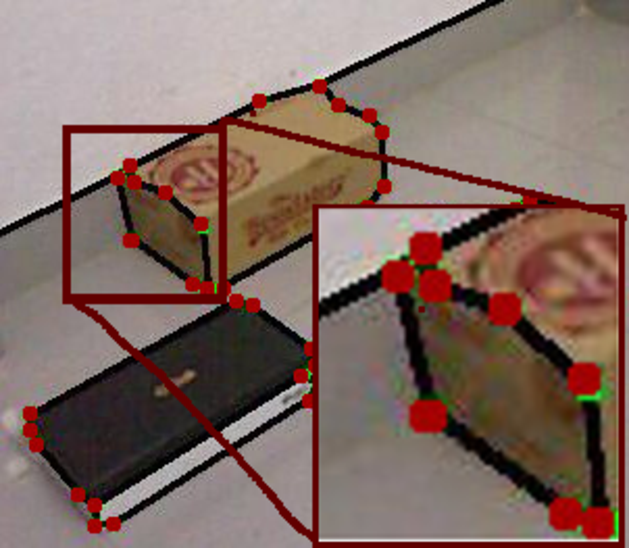
\includegraphics[width=0.27\columnwidth]{images/EdgeLinks.pdf}} \hfill
       \subfigure[Junction Graph]{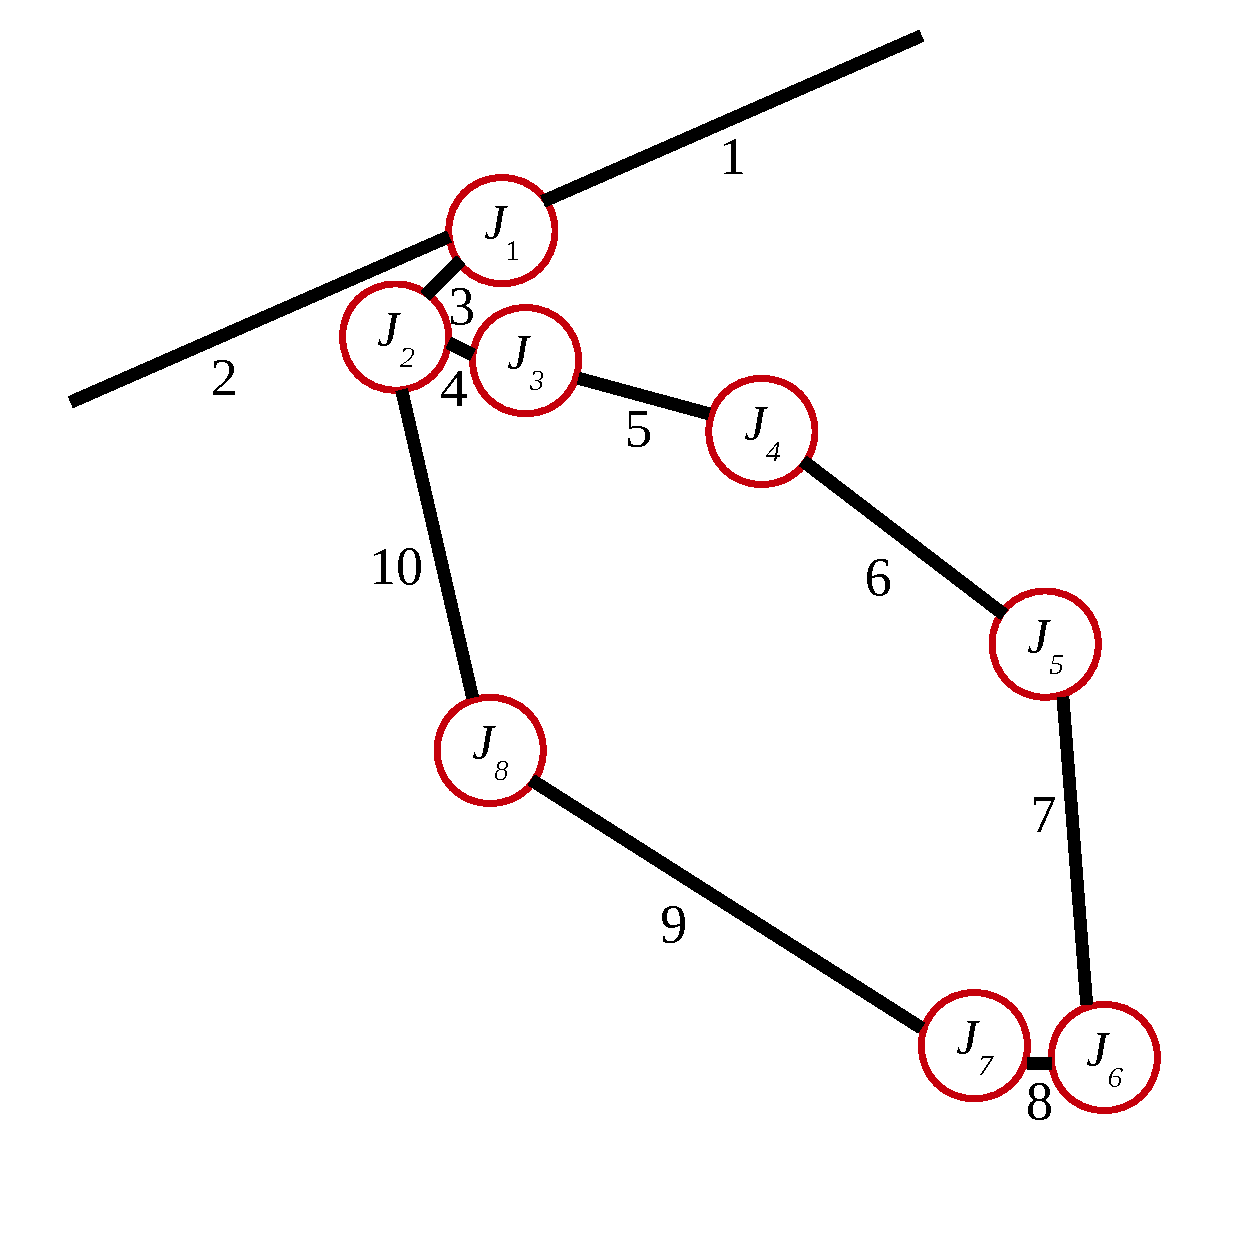
\includegraphics[width=0.27\columnwidth]{images/junctionGraph.pdf}} \hfill
       \subfigure[Contour Graph]{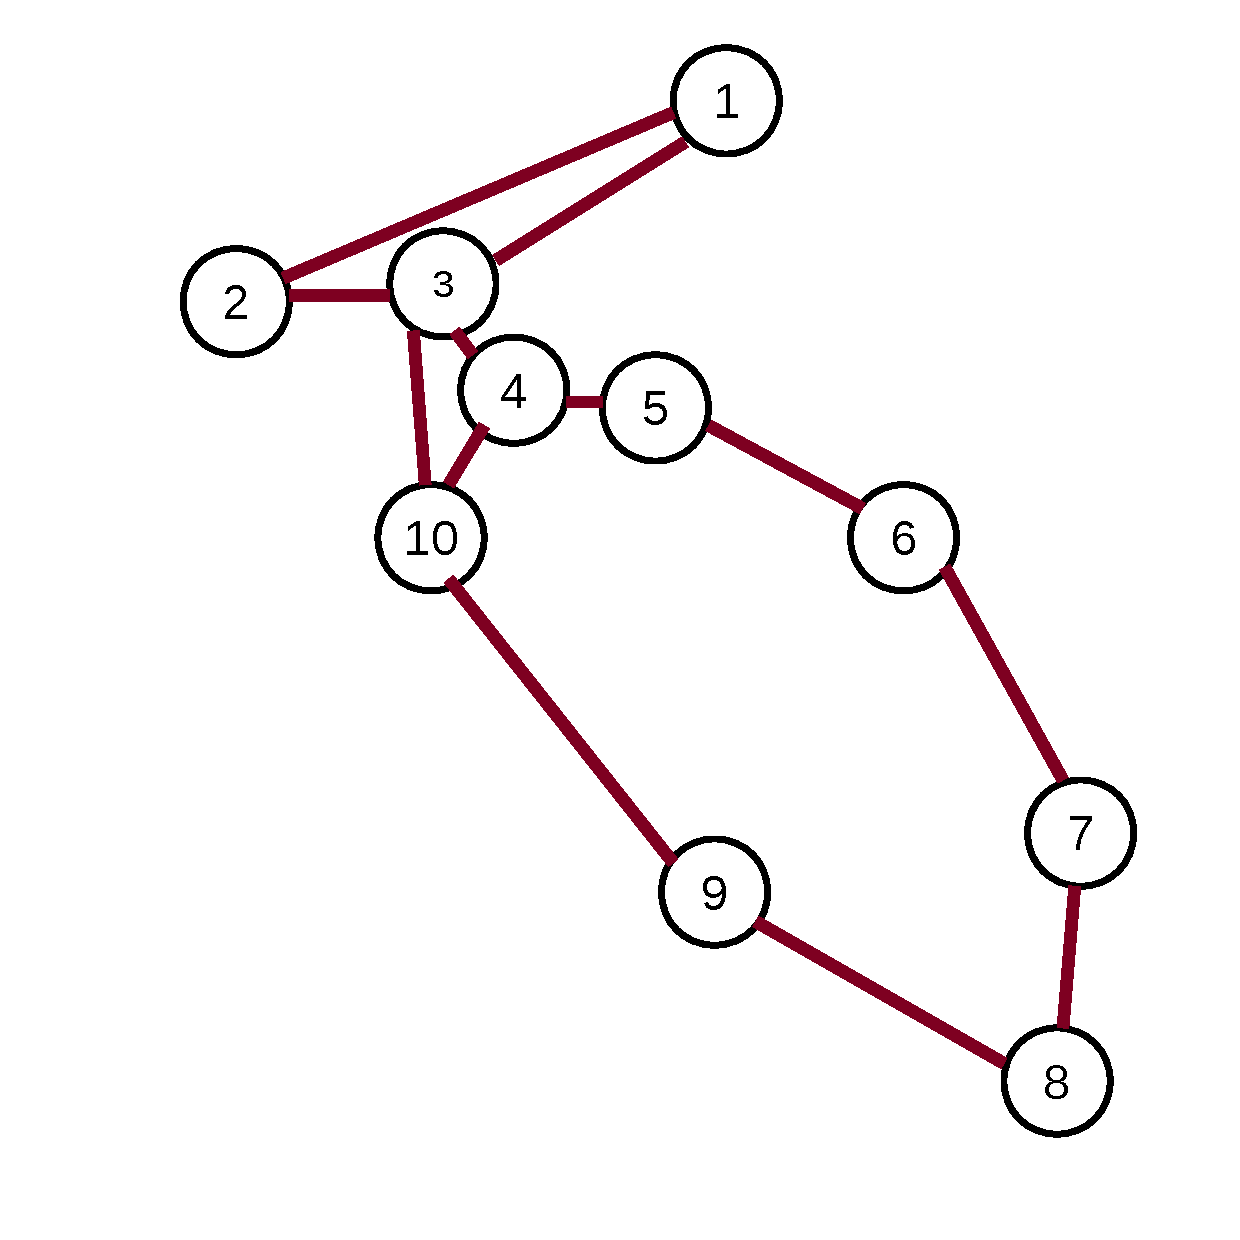
\includegraphics[width=0.27\columnwidth]{images/contourGraph.pdf}} \\
       \caption{\it Contour segments are part of edge links that is bounded by two junctions as shown 
			in (a). In (b), we show a graph where edge junctions are nodes and edge links are edges. In 
			(c), we show a graph with contour segments $c_i$ as nodes and junctions lead to edges between nodes.}
\label{fig:graph_construction}
\end{figure}

To formulate the problem as a labeling problem on an MRF, we need to define unary potentials for
each node $c_i$, as well as the pairwise potentials for every edge in the graph ${\cal G}$.

\subsection{Unary Potentials}

To define the unary potentials of an edge contour $c_i$, we consider the corresponding set of
edge pixels in $c_i$. We define a feature vector for each edge pixel and use a classifier to 
predict its class label. The unary potential of edge contour $c_i$ for label $l$ is 
defined as:
\begin{equation}
\label{unary}
U_l(c_i) = 1 - \frac{N_l}{N_c}
\end{equation}
Here, $N_l$ is the total number of edge pixels on the contour $c_i$ belonging to label $l$. $N_c$ is 
the total number of edge pixels on contour $c_i$. The computation of the feature vector and the 
classification process is described in the following section.

\begin{SCfigure}
       \centering
       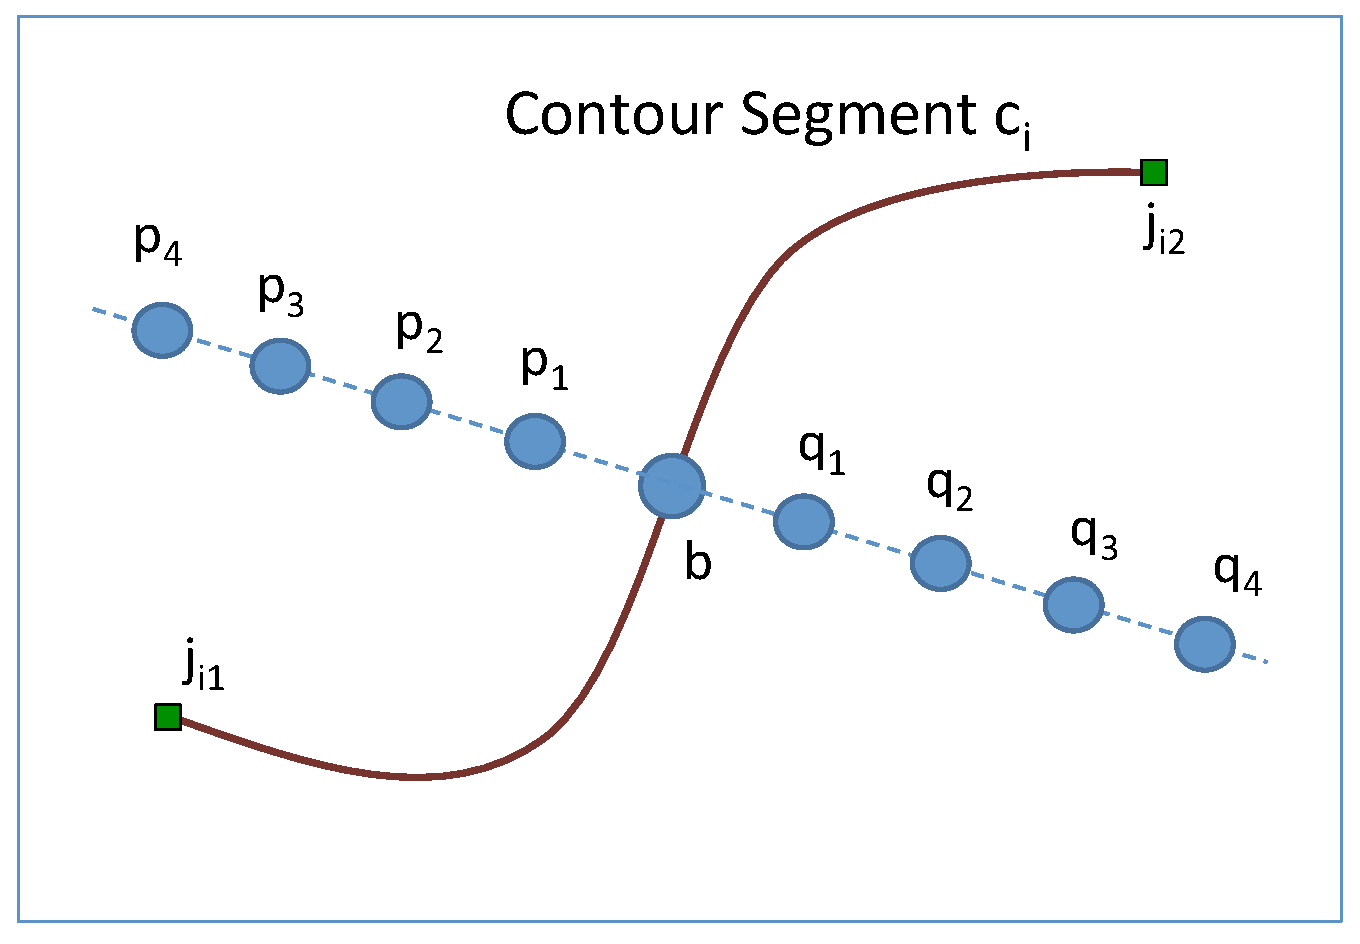
\includegraphics[width=0.40\columnwidth]{images/edgePixels.pdf}
       \caption{\it Edge Pixel Neighborhood: The graph potentials of an edge pixel $b$ are defined based
       on a neighborhood consisting of four pixel on either side of the edge ($p_i$'s and $q_i$'s) on a 
			line perpendicular to the gradient edge direction at $b$.}
\label{fig:edgeNeighbors}
\end{SCfigure}

{\bf The Pixel Classifier:}
Given a contour segment $c_i$, we define its neighborhood properties based on a set of
pixels on either side of the edge as shown in Figure~\ref{fig:edgeNeighbors}. We denote a 
pixel on the contour segment in the image as $b$. We consider $4$ points on either side of 
the edge pixel. These points lie on a line perpendicular to the gradient edge direction at $b$. 
Let the four points on one side be denoted by $(p_1,p_2,p_3,p_4)$ and the other side be 
$(q_1,q_2,q_3,q_4)$. Let $I(p_i)$ denote the RGB color vector at pixel $p_i$.
The corresponding 3D points in the world are denoted using upper 
case letters, $P_i$, $Q_i$ and $B$. The 3D points are obtained using RGBD data. Let $O$ be the 
center of the camera. For a vector $V$, let $<V> = \frac{V}{|V|}$ denote the corresponding 
normalized vector. Let $A.B$ denote the dot product of vectors $A$ and $B$. 
Let ${\cal L}(Q_i,P_j,P_k)$ denote the distance of a point $Q_i$ to the 
3D line joining points $P_j$ and $P_k$. We denote the number of pixels in the neighborhood of 
$b$ with unknown depth values as ${\cal U}(b)$.
	
We briefly describe the role of different elements of the feature vector from the Table~\ref{table:featureVector}.

\begin{table}[h]
\begin{center}
\caption{\it Elements of the feature vector used in pixel-wise edge classifier. Here, the indices 
$i$, $j$ and $k$ vary from 1 to 4.}
\label{table:featureVector}
       \begin{tabular}{|c||c|}
       \hline
        Set Index & Description \\ 
        \hline 
        \hline
				
				1 &
				$<P_i-P_j>.<Q_i-Q_j>$ 
				\\ \hline
				
				2 &
				$\frac{|P_i-Q_i|}{min(|P_i-B|, |Q_i-B|)}$
				\\ \hline
				
				3 &
				$|I(p_i)-I(q_i)|$
				\\ \hline
				
				4 &
				 $<(P_4-B) + (Q_4-B)>.<B-O>$
				\\ \hline
				
				5 & 
				$\frac{|P_i-O|}{|P_{i-1}-O|}$
				\\ \hline
				
				6 &
				${\cal L}(Q_i,P_j,P_k)$
				\\ \hline
				
				7 &
				${\cal U}(b)$
				\\ \hline
				
				8 & 
				$|A-B|,A,B \in \{P_1,..,P_4,B,Q_1,..,Q_4\}$
				\\ \hline
				
				9 & 
				$<P_i-B>.<Q_i-B>$
				\\ \hline
	\end{tabular}
\end{center}
\end{table}


\begin{enumerate}

\item The first set of features denote the dot products based on two vectors on either side of an 
edge pixel. This captures the surface planarity in the neighborhood of an edge pixel. There are six distinct features of this category and are computed from the edge pixel neighborhood (see Figure~\ref{fig:edgeNeighbors}). 
This set of features have high values for planar edge pixels.

\item The second set of features try to capture the depth difference on either side of the edge, 
which helps in finding occlusion edges. The value is expected to be high for occluding edges.

\item The third set captures the normalized color difference between pixels on either side. This 
value is likely to be high for occluding edges.

\item The dot products in the fourth set differentiates between convex and concave labels. 

\item The ratios of distances in the fifth set captures the slopes of surfaces on 
either side from the view point of the camera. This helps in separating convex and concave edges. 
This value would be greater than one for concave and less than one for convex.

\item The sixth set captures the distances from a point to a line. These values are close to zero for planar, 
and nonzero for concave, convex and occluding. For occluding these values are very large.

\item The number of pixels in the neighborhood of an edge with unknown depth values. This number 
is high for occluding edge pixels.

\item The eighth set contains the depth differences between all pairs of points in the set. 

\item The ninth set contains dot products between the pair of vectors originating from $B$ and ending at 
$P_i$ and $Q_i$ respectively.

\end{enumerate}

Given the feature representations of all edge pixels in an image, we train a random forest classifier
with 30 trees that outputs the likelihood for each label. Based on the likelihoods, we identify the class 
label for each pixel.  

\subsection{Inference using graph cuts}

Given the unary and pairwise potentials of each contour segment (node), we will pose the problem
of finding the most likely labels as that of minimizing the total energy over an MRF. A labeling
of the graph, $L$ is defined as an assignment of labels $l_p$ to each node $c_p \in {\cal V}$ in 
the graph ${\cal G}=\{{\cal V},{\cal E}\}$. The data term ${\cal D}(L)$ is a sum
of the unary potentials over all the nodes with respect to the labeling $L$ as shown below:
\begin{equation}
   {\cal D}(L) = \sum_{p=1}^{n} U_{l_p}(c_p)
\end{equation}
The smoothness term ${\cal S}(L)$ is the sum of pairwise potentials over all the neighbors 
$(c_p,c_q) \in {\cal E}$ in the graph ${\cal G}=\{{\cal V},{\cal E}\}$. We use Potts model to define 
the pairwise potential $P_{l_p,l_q}$, which takes a value of 0 for same labels ($l_p=l_q$) and 1 for 
dissimilar ones ($l_p \ne l_q$). The weight factor $W_{l_p,l_q}$ is defined as the cost of assigning 
labels $l_p$ and $l_q$ to any two neighboring nodes $c_p$ and $c_q$. The smoothness terms is shown below:
\begin{equation}
   {\cal S}(L) = \sum_{p,q=1, p \neq q}^{n} W_{l_p,l_q} P_{c_p,c_q}
   \label{eq:datasmooth}
\end{equation}
The total energy $E(L)$ is defined in equation~\ref{eq:E}. The energy function is given by the sum of unary 
and pairwise terms:
\begin{equation}
   \label{eq:E}
   E(L) = \lambda_1  {\cal D}(L) + \lambda_2  {\cal S}(L)
\end{equation}
	
Here, $n$ is the total number of contour segments (nodes) in the graph. The parameters $\lambda_1$ 
and $\lambda_2$ are positive values that control the relative importance of the two terms. For all 
experiments, we use $\lambda_1=1000.0$ and $\lambda_2=12.5$ respectively. The multi-label MRF 
problem is solved using alpha-beta swap~\cite{boykov2001fast}.